\section{Numerical Results}
\label{sec:numerical_results}
To verify the performance of the proposed method we test it on a 3D problem. The reference geometry is a beam  with a square cross-section of size $1 \times 1$ and a length of $10$. The beam is clamped at one end and free at the other. The material properties are set to $E = 4e8$ and $\nu = 0.2$. 
\subsection{Optimal number of modes}
\label{sec:optimal_number_modes}
One of the first steps is clearly to determine the optimal number of modes to be used in the approximation. If we choose too few modes, the approximation will not be accurate enough, but choosing too many modes only increases the complexity of the reduced model, with diminishing returns in terms of accuracy. The figure \ref{fig:optimal_number_modes} shows the error in the approximation of the displacement field as a function of the number of modes used. The error is computed as the Root Mean Square Error (RMSE) between the displacement field computed with the full model and the one computed with the reduced model. The RMSE is defined as:
\begin{equation}
    RMSE = \sqrt{\frac{1}{N}\sum_{i=1}^N (\bm{u}_i^{full} - \bm{u}_i^{reduced})^2},
\end{equation}
where $N$ is the number of nodes in the mesh, $\bm{u}_i^{full}$ is the displacement field computed with the full model and $\bm{u}_i^{reduced}$ is the displacement field computed with the reduced model. The figure shows that the error decreases rapidly with the number of modes used, and then stabilizes around 20 modes. We can see that with 10 modes the error is already below \(10^{-3}\) and with 20 modes the error is below \(10^{-4}\). For our use case, 10 modes are sufficient.
\begin{figure}[H]
    \centering
    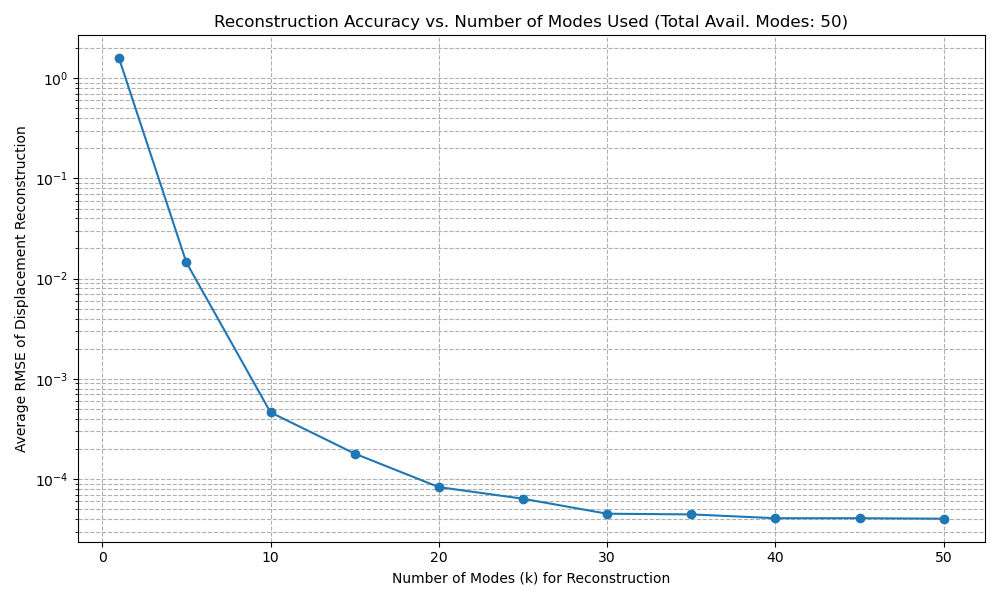
\includegraphics[width=0.7\textwidth]{Images/rmse_vs_modes.png}
    \caption{RMSE of the displacement field as a function of the number of modes used.}
    \label{fig:optimal_number_modes}
\end{figure}


